
\section*{Problema P8.17}

\renewcommand*\thesection{8.17}
\numberwithin{equation}{section}
\numberwithin{figure}{section}

\begin{center}
    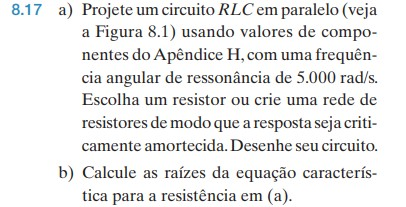
\includegraphics[scale=1.0]{P8.17.jpg}
\end{center}

\subsection*{(a)}

Para o projeto do circuito, fixamos arbitrariamente o indutor selecionado o de $L = 1 \un{mH}$. Para cumprir o
requisito da frequência angular de ressonância ser $\omega_o = 5000\un{rad/s}$, calculamos $C$ através de 

\[ \omega_o = \frac{1}{\sqrt{LC}} \logo C = \frac{1}{\omega_o^2L} \]

\[ C = 40 \un{$\mu$F} \]

Podemos atingir uma capacitância equivalente de $C = 40 \un{$\mu$F}$ usando quatro capacitores de $C_i = 10 \un{$\mu$F}$ em 
paralelo. Para o requisito de ele ser criticamente amortecido, temos que  

\begin{equation}\label{eq:8.17.1}
    \omega_o^2 = \alpha^2
\end{equation}

Expandindo \eqref{eq:8.17.1} conforme as definições,  

\[ \left(\frac{1}{\sqrt{LC}}\right)^2 = \left(\frac{1}{2RC}\right)^2  \]

Isolando $R$,

\[ R = \frac{\sqrt{LC}}{2C}  \]

\[ R = 2.5 \un{$\Omega$}  \]

Podemos obter exatamente uma resistência equivalente de $R = 2.5 \un{$\Omega$}$ com 4 resistores de $R_i = 10 \un{$\Omega$}$
em paralelo.

Assim, temos o circuito projetado na imagem abaixo.

\begin{figure}[hb]
    \centering
    \caption{Circuito RLC projetado. Temos $R = 10 \un{$\Omega$}$ e $C = 10 \un{$\mu$F}$.}
      \centering
      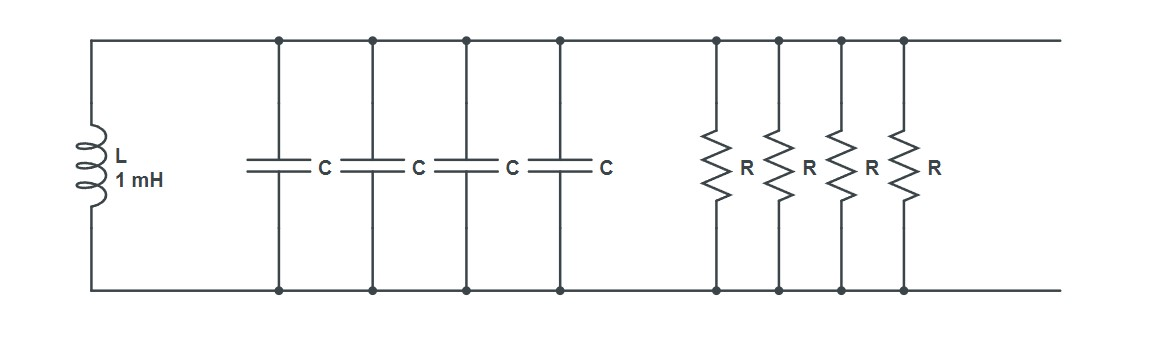
\includegraphics[scale=0.5]{P8.17-Item(a).jpg} \\
    \label{fig:8.17.1}
\end{figure}

\subsection*{(b)}

A equação característica do circuito é   

\begin{equation}\label{eq:8.17.2}
    s^2 + \frac{s}{RC} + \frac{1}{LC} = 0
\end{equation}

Cuja solução é  

\[ s = \frac{-\frac{1}{RC} \pm \sqrt{\Delta}}{2(1)} \]

Note que o circuito já foi projetado para ser criticamente amortecido, e foi possível obter exatamente as resistências
e capacitâncias equivalentes necessárias para obter essa reposta. Logo, temos $\Delta = 0$ e a solução se reduz a

\[ s = \frac{-\frac{1}{RC}}{2} \logo s = -\frac{1}{2RC} \]

Assim, as raízes da equação característica são  

\[ \boxed{s_1 = s_2 = -5000 \un{rad/s} }  \]

